%%%%%%%%%%%%%%%%%%%%%%%%%%%%%%%%%%%%%%%%%%%%%%%%%%%%%%%%
% Este é um documento que servirá de modelo para
% os relatórios feitos na disciplina Laboratório de Circuitos Lógicos
% 2020-2
%%%%%%%%%%%%%%%%%%%%%%%%%%%%%%%%%%%%%%%%%%%%%%%%%%%%%%%%%

%%%%%%%%%%%%%%%%%%%%%%%%%%%%%%%%%%%%%%%%%%%%%%%%%%%%%%%%%
% Use os diferentes diretórios para colocar os relatórios de cada experimento, deste modo vc consegue manter um histórico e todo material organizado em apenas um local.
% Lembre-se de mudar o Main Document no Menu!!!

\documentclass[12pt]{article}

\usepackage{sbc-template}
\usepackage[brazil,american]{babel}
\usepackage[utf8]{inputenc}

\usepackage{graphicx}
\usepackage{url}
\usepackage{float}
\usepackage{listings}
\usepackage{color}
\usepackage{todonotes}
\usepackage{algorithmic}
\usepackage{algorithm}
\usepackage{hyperref}
\usepackage{amsmath}
\usepackage{graphicx}
\usepackage{array}
\usepackage{mwe}
\usepackage{pythonhighlight}
\usepackage[shortlabels]{enumitem}

\usepackage{xcolor}
\usepackage{listings}
\usepackage[electronic]{ifsym}
\definecolor{vgreen}{RGB}{104,180,104}
\definecolor{vblue}{RGB}{49,49,255}
\definecolor{vorange}{RGB}{255,143,102}

\lstdefinestyle{verilog-style}
{
    language=Verilog,
    basicstyle=\small\ttfamily,
    keywordstyle=\color{vblue},
    identifierstyle=\color{black},
    commentstyle=\color{vgreen},
    numbers=left,
    numberstyle=\tiny\color{black},
    numbersep=10pt,
    tabsize=8,
    moredelim=*[s][\colorIndex]{[}{]},
    literate=*{:}{:}1
}

\makeatletter
\newcommand*\@lbracket{[}
\newcommand*\@rbracket{]}
\newcommand*\@colon{:}
\newcommand*\colorIndex{%
    \edef\@temp{\the\lst@token}%
    \ifx\@temp\@lbracket \color{black}%
    \else\ifx\@temp\@rbracket \color{black}%
    \else\ifx\@temp\@colon \color{black}%
    \else \color{vorange}%
    \fi\fi\fi
}
\makeatother

\usepackage{trace}

\sloppy


\title{Projeto Final\\
ZeptoProcessador-III de 16 Bits}

\author{Matheus Cardoso de Souza, 202033507\\
        Ualiton Ventura da Silva, 202033580\\
        Grupo G42
}

%%%% LEMBRE-SE DE MUDAR O GRUPO NA LINHA ABAIXO!!!!! %%%%%%
\address{Dep. Ciência da Computação -- Universidade de Brasília (UnB)\\
  CIC0231 - Laboratório de Circuitos Lógicos
  \email{matheus-cardoso.mc@aluno.unb.br, 202033580@aluno.unb.br}
}

\begin{document}
\maketitle

\selectlanguage{american}
 \begin{abstract}
   The present report will show a detailed description of all the needed process
   to build a processor, one of the most important logic circuits today. Also,
   the processors' functions will be assessed when submitted to execution of
   arbitrary code, therefore showing their generality in a wide variety of
   activities.
 \end{abstract}

\selectlanguage{brazil}
 \begin{resumo}
   O presente relatório apresentará uma descrição detalhada de todos os
   processos que abrangem a construção de um processador, um dos circuitos
   lógicos mais importantes na atualidade. Também será abordado o comportamento
   do processador quando submetido à execução de códigos arbitrários inseridos
   pelo usuário, dessa forma demonstrando a generalidade para uso em diversas
   atividades.
 \end{resumo}


\section{Introdução}\label{sec:Introducao}

Na atualidade, com o advento dos computadores, um dos circuitos mais improtantes
para a sociedade moderna se tornou os processadores. Tais circuitos
apresentam-se como um dos mais complexos na área de circuitos lógicos. Para o
presente relatório, entretanto, abordaremos a construção de um relativamente
simples, contendo apenas um registrador de instruções, uma memória de instruções
que armazena instruções de $32$ \emph{bits}, e um banco de registradores de $16$
registradores contendo $16$ bits cada.

\subsection{Objetivos}\label{sec:Objetivos}

Temos como objetivo neste projeto final desenvolvermos um processador (chamado
\emph{ZeptoProcessador-III}), com as características de ser um processador de
$16$ \emph{bits}, com memória de instruções própria, suportando instruções de
$32$ \emph{bits}. O processador terá um conjunto de $13$ instruções, a saber:
\{\emph{add}, \emph{subi}, \emph{andi}, \emph{ori}, \emph{xori}, \emph{beq},
\emph{bne}, \emph{ble}, \emph{bleu}, \emph{bgt}, \emph{bgtu}, \emph{jal} e
\emph{jalr}\}

\subsection{Materiais}\label{sec:Materiais}

Em função da natureza do ensino a distância, os presentes experimentos não foram
realizados usando-se materiais e equipamentos físicos, mas sim emulados por meio
do software
\href{https://www.digitalelectronicsdeeds.com/downloads.html}{Deeds}.

A seguir estão enumerados os materiais utilizados:
\begin{itemize}
    \item Software Deeds
    \item Portas lógicas
    \begin{itemize}
      \item Portas Lógicas \emph{AND}
      \item Portas Lógicas \emph{NAND}
      \item Portas Lógicas \emph{NOR}
      \item Portas Lógicas \emph{OR}
    \end{itemize}
    \item \emph{Clocks}
    \item Display de saída de 1 bit
    \item Display de saída de 8 Segmentos
    \item Memórias \emph{ROM}
    \item Multiplexadores
    \item Unidades Lógico-Aritméticas - \emph{ULA}s
\end{itemize}

\section{Procedimentos}\label{sec:Procedimentos}
% \setcounter{subsection}{-1}

Como o processador é um circuito complexo, optou-se por abordar a implementação
de cada bloco lógico de forma separada, e, posteriormente, mostrar como esses
blocos individuais podem ser integrados para resultar em um circuito funcional.
Começaremos demonstrando a montagem do circuito do principal registrador do
processador, o registrador \emph{PC}.

% 2.1
\subsection{Montagem do Circuito do Processador \emph{PC}}\label{sec:2.1}

Todo processador deve possuir um registrador principal que sirva de ``maestro''
do circuito como um todo. Este processador, também chamado de processador de
instruções, tem a funcionalidade de armazenar a instrução que está atualmente
sendo decodificada e/ou executada. Como o processador ZeptoProcessador-III é bem
simples, precisamos de apenas um registrador desse tipo para obtermos os
resultados esperados. Entretanto, em processadores mais modernos e complexos
(vide~\cite{Instruction_register}), vários processadores de instrução podem ser
acoplados para formarem uma \emph{pipeline} de instruções, onde cada parte da
\emph{pipeline} é responsável por parte do processo de decodificação, preparação
ou execução das instruções passadas.

Como é possível observar pela
imagem~\ref{fig:circuit__instruction_register.png}, o registrador de instruções
(no centro da imagem), tem como input o resultado do último ciclo de instruções.
Além disso, está diretamente ligado ao sinal de clock que sincroniza todos os
componentes do processador, e também a um sinal de reset (na imagem com o nome
de \emph{Start}). Seu output é utilizado como entrada para a memória de
instruções (para obter a próxima intrução que deve ser processada), e também
utilizada em um somador (aqui não mostrado devido à distância entre o
registrador e o somador), para calcular o próximo endereço de instrução a ser
processado.

\begin{figure}[H]
    \centering
    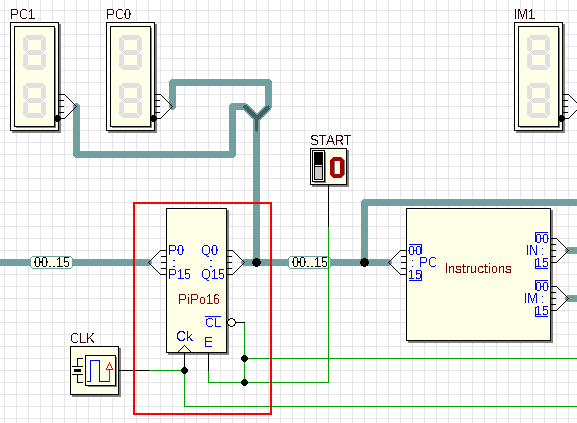
\includegraphics[width=.9\textwidth]{Projeto/images/circuit__instruction_register.png}
    \caption{Zoom no Registrador de Instruções}\label{fig:circuit__instruction_register.png}
\end{figure}

O processador ZeptoProcessador-III segue a mesma ideia de execução do
processador \emph{MIPS} apresentado na figura~\ref{fig:circuit__MIPS.png}
(fonte:~\cite{Digital_Design}). Então é possível ver todas as ligações
relevantes relacionadas ao registrador de instruções.

\begin{figure}[H]
    \centering
    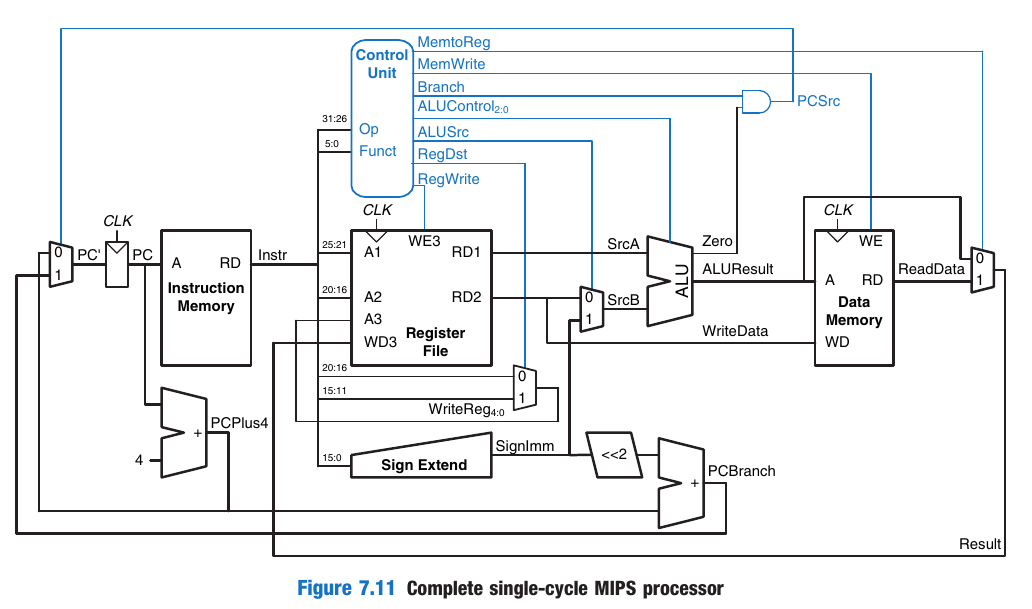
\includegraphics[width=.9\textwidth]{Projeto/images/circuit__MIPS.png}
    \caption{Overview esquemático do processador \emph{MIPS}}\label{fig:circuit__MIPS.png}
\end{figure}

% 2.2
\subsection{Montagem do Circuito da Memória de Instruções}\label{sec:2.2}

Como foi possível observar no circuito do registrador de instruções, o output
daquele circuito se ligava à memória de instruções. Tal componente de um
processador server para armazenar as instruções que um usuário do processador
deseja que este execute. Dessa forma, o processador se torna \emph{programável}.

No ZeptoProcessador-III, a memória de instruções é implementada utilizando-se a
memória ROM. Ela é uma memória somente de leitura, de rápido acesso. Tal tipo de
memória foi muito utilizada por exemplo em cartuchos de \emph{video-games},
\emph{CD}s e afins (para maiores informações sobre essa tecnologia,
consultar~\cite{ROM_memory})

Sua implementação no circuito integrado do processador é dada conforme a
imagem~\ref{fig:circuit__ROM_memory.png}. Pela figura, é possível observar que
existem duas memórias ROM separadas, que recebem como input o endereço produzido
pelo registrador de instruções. O uso de duas memórias ROM separadas se dá
devido ao fato de que, segundo as especificações do ZeptoProcessador-III, a
memória de instruções deve ser capaz de armazenar instruções de $32$
\emph{bits}. Entretanto, como a maior memória ROM disponível no \emph{Deeds} é
de $16$ \emph{bits}, foi utilizado uma memória ROM para armazenar os $16$
\emph{bits} menos significativos, e outra ROM para os outros $16$ \emph{bits}
mais significativos.

\begin{figure}[H]
    \centering
    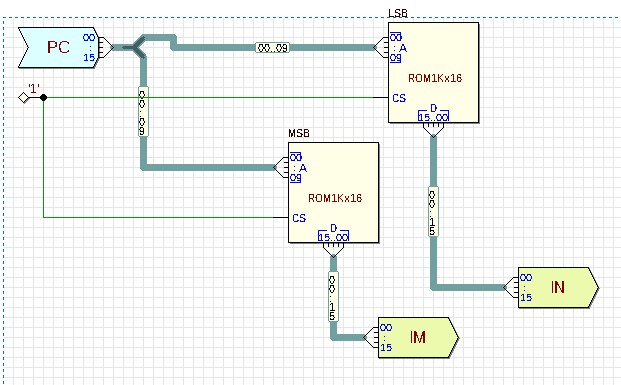
\includegraphics[width=.9\textwidth]{Projeto/images/circuit__ROM_memory.png}
    \caption{Overview da Memória de Instruções}\label{fig:circuit__ROM_memory.png}
\end{figure}

% 2.3
\subsection{Montagem do Circuito do Banco de Registradores}\label{sec:2.3}

O próximo bloco de circuito lógico necessário para um processador funcional é o
\emph{Banco de Registradores}. Tal circuito possibilita o armazenamento de dados
durante a operação do processador, servindo como memória para manipulação de
variáveis e controle de estados.

O ZeptoProcessador-III possui como especificação um banco de registradores
contendo $16$ registradores de $16$ \emph{bits} cada. Além disso,
esquematicamente o banco de registradores funciona da sequinte forma: $3$ canais
de input sinalizam respectivamente o endereço de leitura dos registradores
\emph{Ra}, \emph{Rb} e o endereço de escrita do registrador \emph{Rd}. O banco
de registradores também possui um canal com $16$ \emph{bits} que corresponde aos
dados de escrita, o sinal de \emph{clock}, um sinal para informar se o banco de
registradores deve escrever os dados de escrita no registrador \emph{Rd}, um
sinal de \emph{reset} (que faz com que todos os registradores no banco assumam o
valor $0$), e por fim também possui dois canais de saída de dados \emph{Sa} e
\emph{Sb} que são os dados de leitura dos registradores nos endereços \emph{Ra}
e \emph{Rb}, respectivamente. A figura~\ref{fig:diagram__register_file.png}
(fonte:~\cite{Diagram_Register_file}) mostra esquematicamente como opera um
banco de registradores.

\begin{figure}[H]
    \centering
    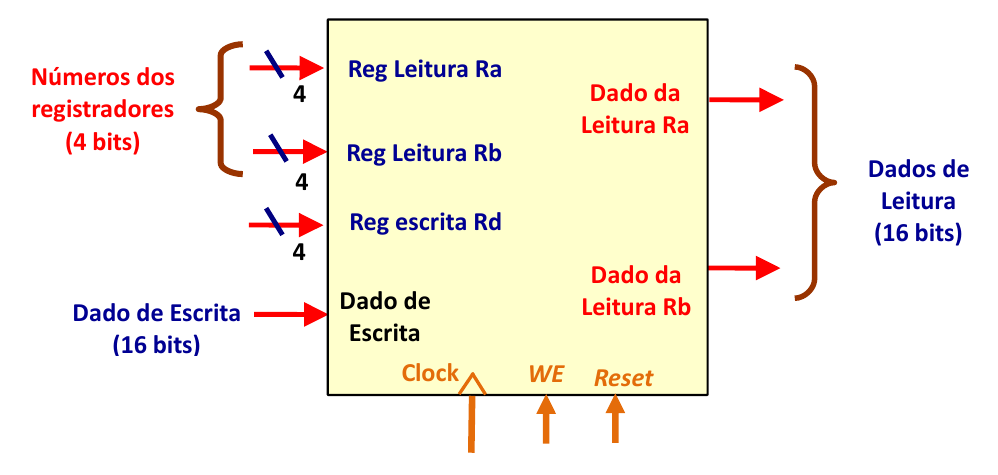
\includegraphics[width=.9\textwidth]{Projeto/images/diagram__register_file.png}
    \caption{Esquema do funcionamento de um Banco de Registradores}\label{fig:diagram__register_file.png}
\end{figure}

E, finalmente, na figura~\ref{fig:circuit__register_file.png} é possível ver
como foi organizado o banco de registradores do ZeptoProcessador-III. Por ser um
circuito muito grande, as figuras~\ref{fig:circuit__register_file_1.png}
e~\ref{fig:circuit__register_file_2.png} mostram, respectivamente, mais
detalhadamente os circuito dos registradores e dos selecionadores de canais
valendo-se de multiplexadores. Novamente, por uma limitação dos blocos
pré-existentes no \emph{Deeds}, a seleção de canais foi feita com dois
multiplexadores de $8$ canais e posteriormente com um multiplexador de $2$
canais devido a ausência de um multiplexador que contenha diretamente $16$
canais.

\begin{figure}[H]
    \centering
    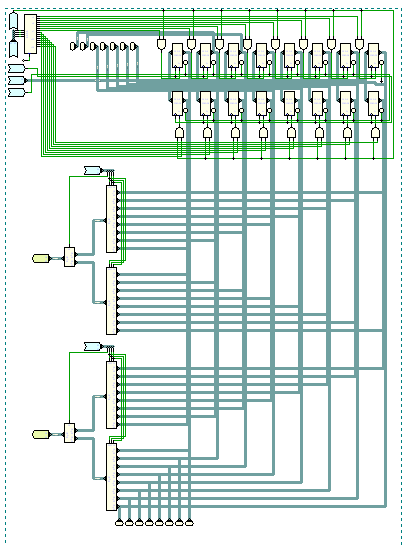
\includegraphics[width=.9\textwidth]{Projeto/images/circuit__register_file.png}
    \caption{Montagem do Banco de Registradores}\label{fig:circuit__register_file.png}
\end{figure}

\begin{figure}[H]
    \centering
    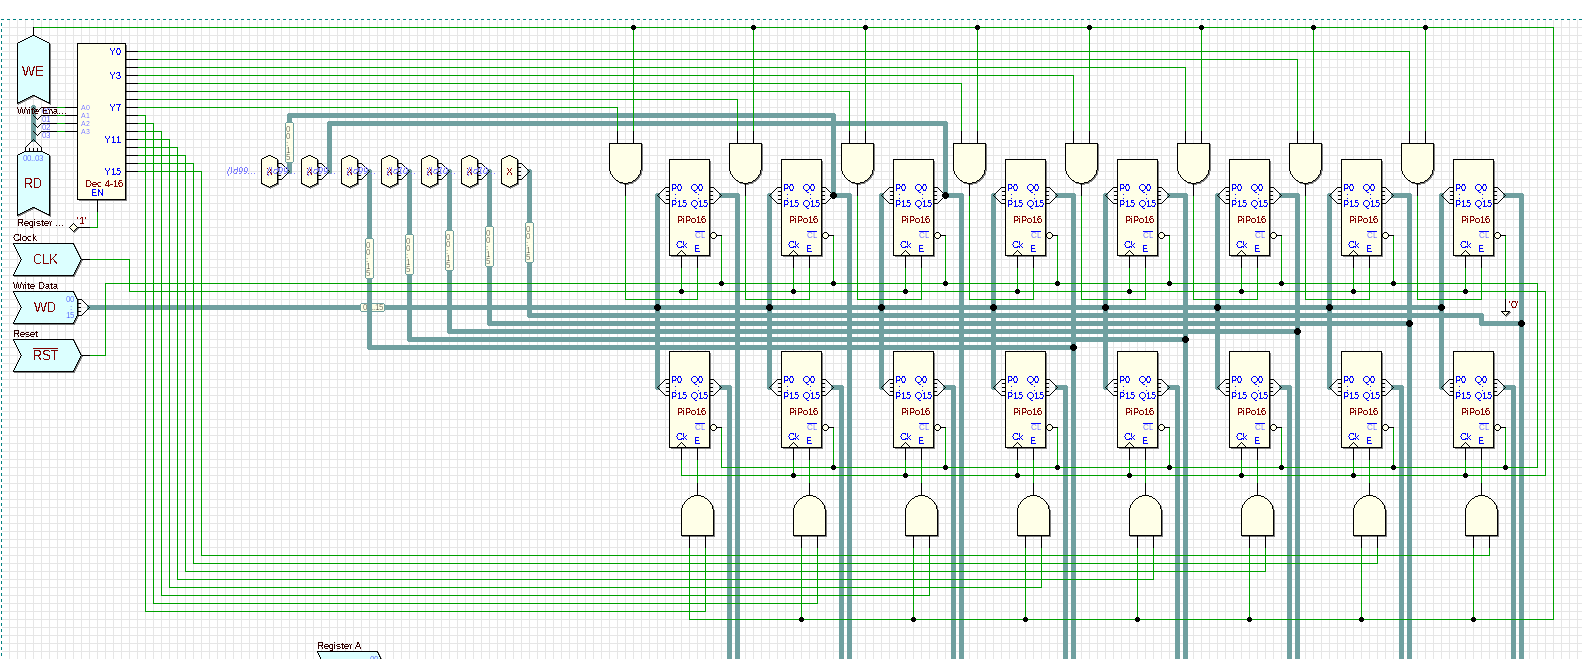
\includegraphics[width=.9\textwidth]{Projeto/images/circuit__register_file_1.png}
    \caption{Zoom nos registradores do banco}\label{fig:circuit__register_file_1.png}
\end{figure}

\begin{figure}[H]
    \centering
    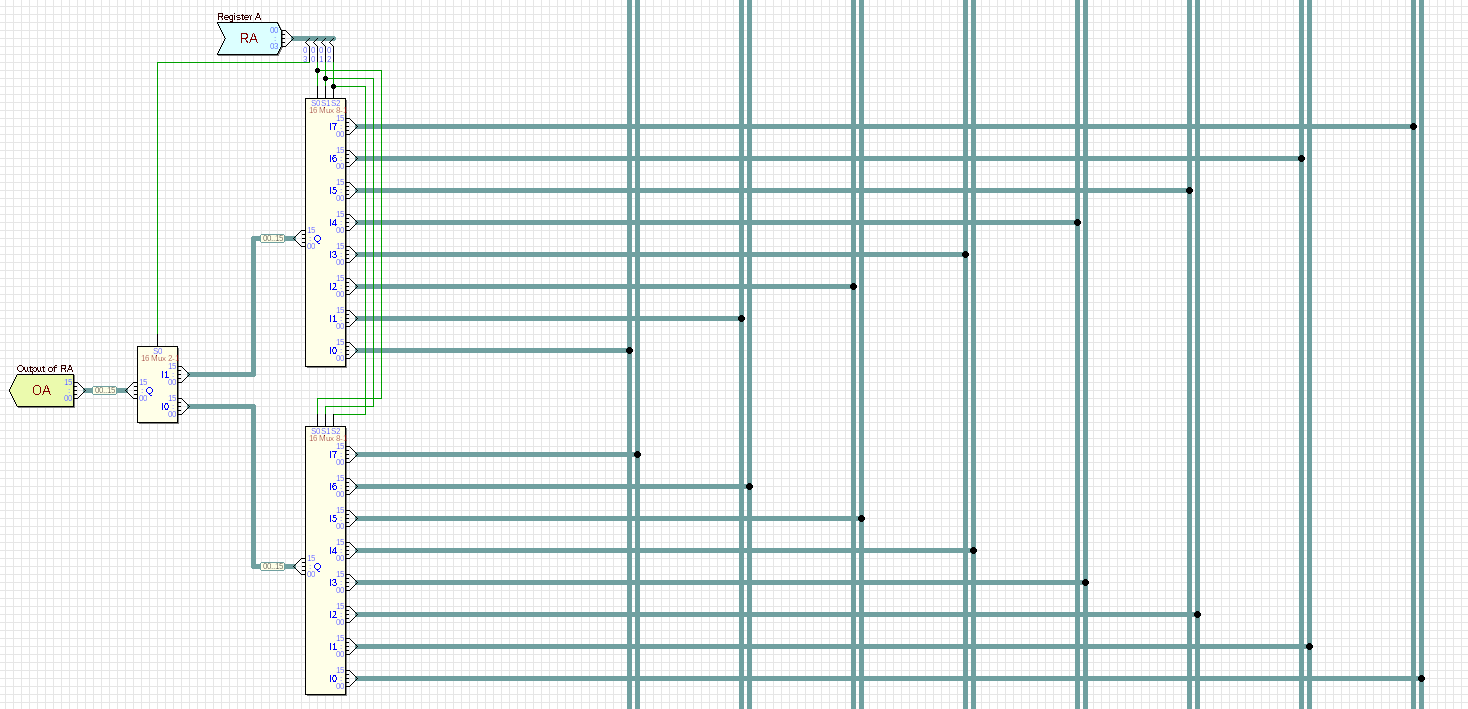
\includegraphics[width=.9\textwidth]{Projeto/images/circuit__register_file_2.png}
    \caption{Zoom no seletor de canais}\label{fig:circuit__register_file_2.png}
\end{figure}


% 2.4
\subsection{Montagem do Unidade Lógico Aritmética}\label{sec:2.4}

A Unidade Lógico Aritmética (\emph{ULA}), é um circuito indispensável a qualquer
processador, pois é ela que permite por exemplo operações de soma, subtração,
desvios condicionais e saltos incondicionais.

No ZeptoProcessador-III, a ULA foi implementada da seguinte forma (que pode ser
visualizada na figura~\ref{fig:circuit__ula.png})

\begin{figure}[H]
    \centering
    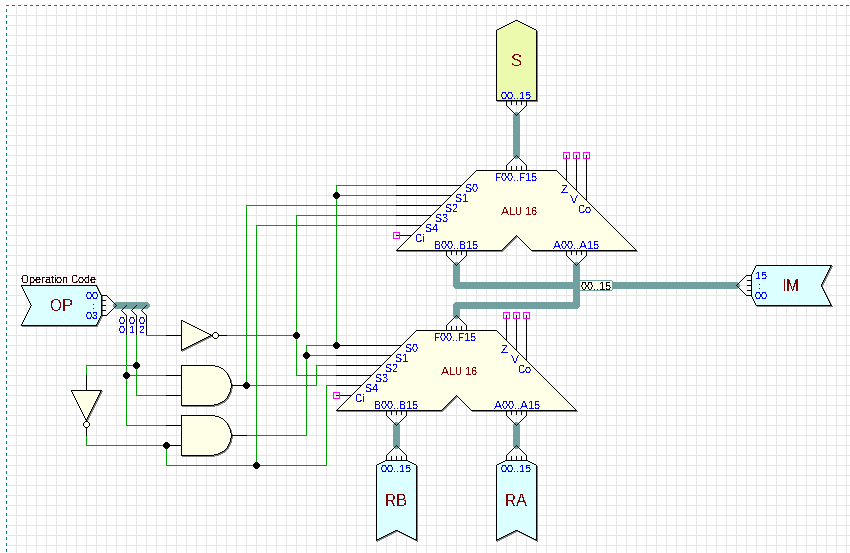
\includegraphics[width=.9\textwidth]{Projeto/images/circuit__ula.png}
    \caption{Montagem do circuito comparador de números}\label{fig:circuit__ula.png}
\end{figure}

\subsection{Montagem do Circuito do Comparador de Números}\label{sec:2.5}

Uma das funcionalidades mais importantes de se ter em um processador é a
capacidade de chegagem de (des)igualdade entre números. Para implementarmos tal
funcionalidade em um processador faz-se necessário a criação de um bloco que
permita comparar, a nível de \emph{bits}, se um determinado número é igual,
maior ou menor que outro. Como existem duas possibilidades de tratamento de
números (números \emph{com} e \emph{sem} sinal), o circuito necessita ainda de
um tratamento especial para tal condição.

Dessa forma, no ZeptoProcessador-III foi implementado um circuito com o seguinte
esquema (que pode ser visualizado na figura~\ref{fig:circuit__comparator.png}):

\begin{figure}[H]
    \centering
    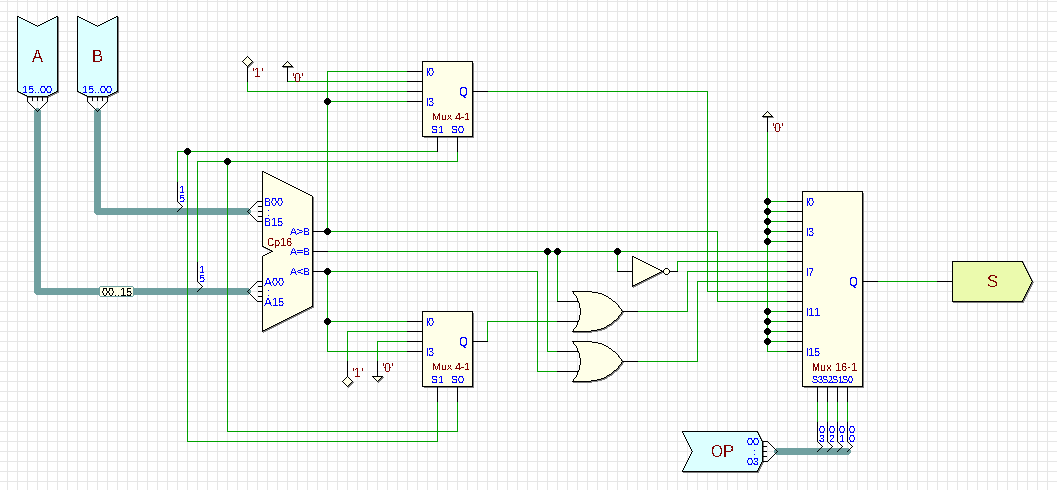
\includegraphics[width=.9\textwidth]{Projeto/images/circuit__comparator.png}
    \caption{Montagem do circuito comparador de números}\label{fig:circuit__comparator.png}
\end{figure}

\subsection{Montagem do Circuito do Bloco de Controle}\label{sec:2.6}

Como é possível perceber na figura~\ref{fig:circuit__MIPS.png}, um dos circuitos
lógicos importantes do processador é o bloco de controle. Ele é responsável por
interpretar as instruções lidas da memória de instruções. Dessa forma, há um
mapeamento de determinada instrução para uma execução específica do processador.

Tal bloco, no ZeptoProcessador-III, foi implementado da seguinte forma (possível
de ser visualizado na figura~\ref{fig:circuit__control.png})

\begin{figure}[H]
    \centering
    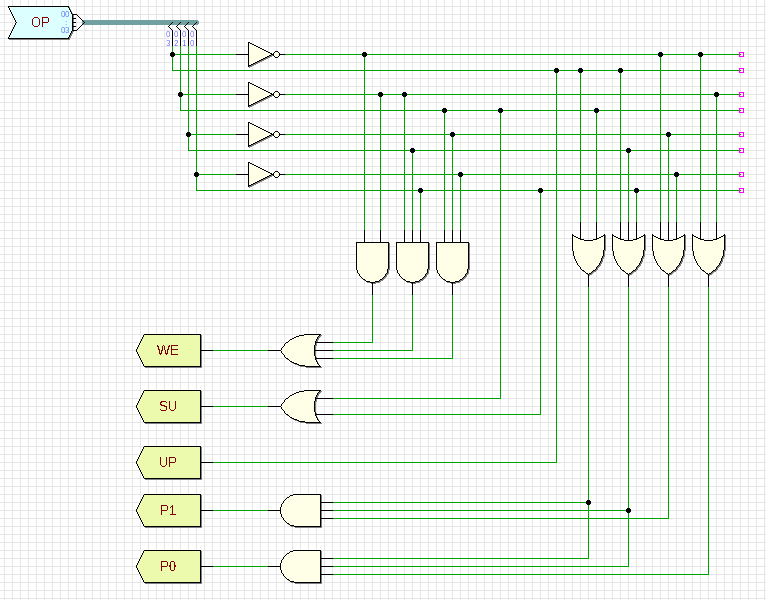
\includegraphics[width=.9\textwidth]{Projeto/images/circuit__control.png}
    \caption{Montagem do Bloco de Controle}\label{fig:circuit__control.png}
\end{figure}

\subsection{Montagem dos Sinais de Monitoramento}\label{sec:2.4}

Por fim, uma característica importante de se adicionar ao ZeptoProcessador-III
são sinais de monitoramento, para uma melhor capacidade de avaliar se o circuito
se comporta de fato como esperado. Na figura~\ref{fig:circuit__signals.png} é
possível ver os diversos sinais de monitoramento inseridos no circuito para uma
melhor visualização de seu comportamento durante operação.

\begin{figure}[H]
    \centering
    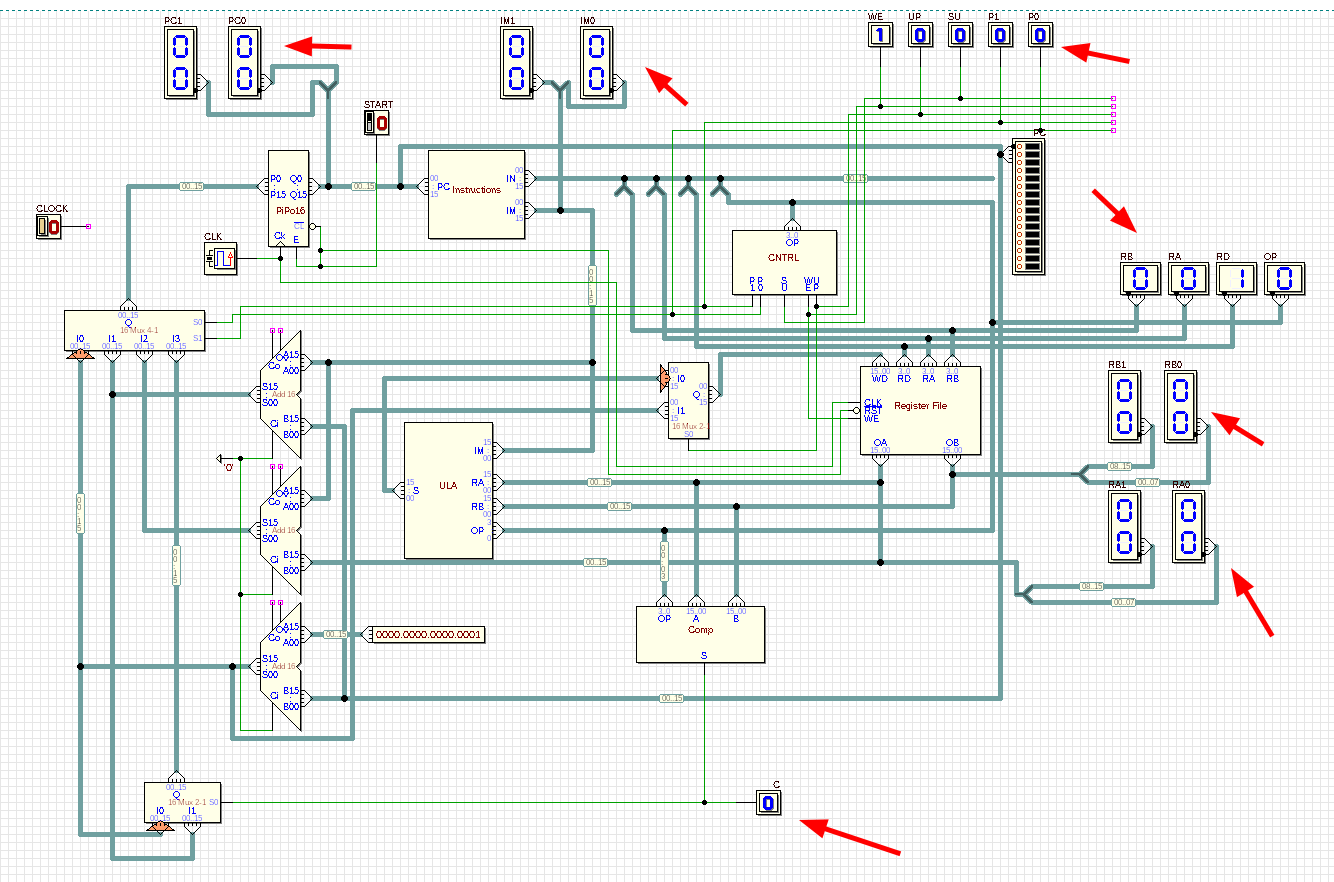
\includegraphics[width=.9\textwidth]{Projeto/images/circuit__signals.png}
    \caption{Montagem dos Sinais de Monitoramento}\label{fig:circuit__signals.png}
\end{figure}


\section{Execução de Programas no ZeptoProcessador-III}\label{sec:programs}

\subsection{Multiplicação de Números sem Sinal}\label{sec:programs:multu}

Para o primeiro programa proposto no projeto, faremos um que multiplique dois
números sem sinal, e retorne o valor da multiplicação no registrador \emph{R1}.
Os valores de input para o programa serão carregados nos registradores \emph{R2}
e \emph{R3}, com valores de $8$ e $5$, respectivamente. O resultado esperado da
multiplicação será $8 \cdot 5 = 40$, que, em hexadecimal, corresponde a
$0x0028$.

O código do programa, e seus respectivos comentários, podem ser encontrados na
tabela~\ref{tab:programs:multu}.

\begin{table}[H]
    \centering
    \caption{Código para o programa \textbf{Multu}}
    \begin{tabular}{|l|l|l|l|}\hline
        \textbf{Endereço} & \textbf{Código Hexadecimal} & \textbf{Instrução} & \textbf{Comentário} \\\hline
        0x0000       & 0x0000 0010 & addi R1,R0,R0,0 & R1 = 0 ;; Resultado           \\\hline
        0x0001       & 0x0008 0020 & addi R2,R0,R0,8 & R2 = 8                        \\\hline
        0x0002       & 0x0005 0030 & addi R3,R0,R0,5 & R3 = 5                        \\\hline
        0x0003       & 0x0002 00FB & jal R15,Proc    & R15 = 0x0004; PC=Proc         \\\hline
        0x0004 Fim:  & 0x0000 1105 & beq R1,R1,0     & j Fim ;; mostra R1            \\\hline
        0x0005 Proc: & 0x0000 0040 & addi R4,R0,R0,0 & R4 = 0 ;; instantiate counter \\\hline
        0x0006 Loop: & 0x0000 2110 & addi R1,R1,R2,0 & R1 += R2                      \\\hline
        0x0007       & 0x0001 0440 & addi R4,R4,R0,1 & R4 += 1                       \\\hline
        0x0008       & 0xFFFE 3406 & bne  R4,R3,Loop & if (R4 \!= R3) goto Loop      \\\hline
        0x0009       & 0x0000 0F0C & jalr R0,R15,0   & Retorna resultado em R1       \\\hline
    \end{tabular}\label{tab:programs:multu}
\end{table}

Para a demonstração do programa funcionando, por favor conferir o vídeo no link:
\href{https://youtu.be/NygIUTYyUNY}{https://youtu.be/NygIUTYyUNY}

E, como requisitado, o diagrama de onda do programa pode ser visto na
figura~\ref{fig:program__multu_wave.png}. O processador conseguiu executar o
presente programa na máxima frequência de $4.35MHz$. Qualquer outra frequência
mais rápida que essa resulta em falha no funcionamento, e toda frequência menor
que essa resulta em um resultado sub-ótimo.

\begin{figure}[H]
    \centering
    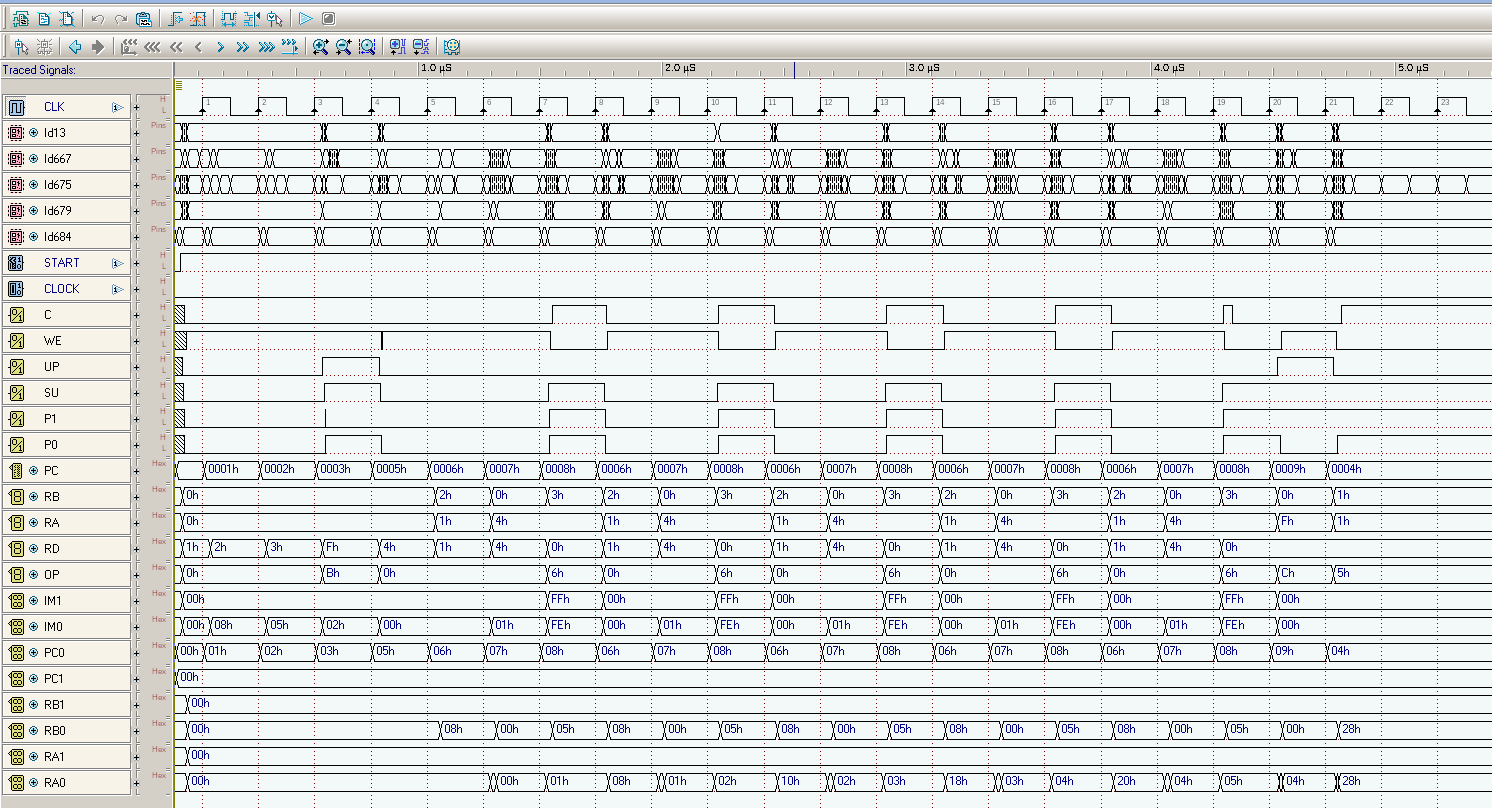
\includegraphics[width=.9\textwidth]{Projeto/images/program__multu_wave.png}
    \caption{Diagrama de onda para o programa Multu}\label{fig:program__multu_wave.png}
\end{figure}

\subsection{Multiplicação de Números com Sinal}\label{sec:programs:mult}

Agora, para o programa de multiplicação de números com sinal, o programa
proposto realiza a multiplicação de dois números com sinal, e retorna o valor da
multiplicação no registrador \emph{R1}. Os valores de input para o programa
serão carregados nos registradores \emph{R2} e \emph{R3}, com valores de $-2$ e
$5$, respectivamente. O resultado esperado da multiplicação será
$-2 \cdot 5 = -10$, que, em hexadecimal, corresponde a $0xFFF6$.

O código do programa, e seus respectivos comentários, podem ser encontrados na
tabela~\ref{tab:programs:mult}.

\begin{table}[H]
    \centering
    \caption{Código para o programa \textbf{Mult}}
    \begin{tabular}{|l|l|l|l|}\hline
        \textbf{Endereço} & \textbf{Código Hexadecimal} & \textbf{Instrução} & \textbf{Comentário}\\\hline
        0x0000        & 0x0000 0010 & addi R1,R0,R0,0      & R1 = 0 ;; Resultado            \\\hline
        0x0001        & 0xFFFE 0020 & addi R2,R0,R0,-2     & R2 = -2                        \\\hline
        0x0002        & 0x0005 0030 & addi R3,R0,R0,5      & R3 = 5                         \\\hline
        0x0003        & 0x0002 00FB & jal  R15,Proc        & R15 = 0x0004; PC=Proc          \\\hline
        0x0004 Fim:   & 0x0000 1105 & beq  R1,R1,0         & j Fim ;; mostra R1             \\\hline
        0x0005 Proc:  & 0x0000 0040 & addi R4,R0,R0,0      & R4 = 0 ;; counter              \\\hline
        0x0006        & 0x8000 0050 & addi R5,R0,R0,0x8000 & R5 (is a mask)                 \\\hline
        0x0007        & 0xFFFF 5262 & andi R6,R2,R5,0xFFFF & R6 == 0x08000 ?                \\\hline
        0x0008        & 0x0004 5606 & bne  R6,R5,R2end     & R6 is a result of a mask       \\\hline
        0x0009        & 0x0001 4040 & addi R4,R0,R4,1      & Increment count of odd numbers \\\hline
        0x000A        & 0xFFFF 0224 & xori R2,R2,R0,0xFFFF & One's compelemnt for R2        \\\hline
        0x000B        & 0x0001 0220 & addi R2,R2,R0,1      & Two's compelemnt for R2        \\\hline
        0x000C R2end: & 0xFFFF 5362 & andi R6,R3,R5,0xFFFF & R6 == 0x08000 ?                \\\hline
        0x000D        & 0x0004 5606 & bne  R6,R5,R3end     & R6 is a result of a mask       \\\hline
        0x000E        & 0x0001 0440 & addi R4,R4,R0,1      & Increment count of odd numbers \\\hline
        0x000F        & 0xFFFF 0334 & xori R3,R3,R0,0xFFFF & One's compelemnt for R3        \\\hline
        0x0010        & 0x0001 0330 & addi R3,R3,R0,1      & Two's compelemnt for R3        \\\hline
        0x0011 R3end: & 0x0000 0070 & addi R7,R0,R0,0      & R7 = 0 ;; loop counter         \\\hline
        0x0012 Loop:  & 0x0000 2110 & addi R1,R1,R2,0      & R1 += R2                       \\\hline
        0x0013        & 0x0001 0770 & addi R7,R7,R0,1      & R7 += 1                        \\\hline
        0x0014        & 0xFFFE 3706 & bne  R7,R3,Loop      & if (R7 \!= R3) goto Loop       \\\hline
        0x0015        & 0x0001 0060 & addi R6,R0,R0,1      & R6 = 1                         \\\hline
        0x0016        & 0x0003 6406 & bne  R4,R6,Ok        & if (R4 \!= R6) goto Ok         \\\hline
        0x0017        & 0xFFFF 0114 & xori R1,R1,R0,0xFFFF & One's complement for R1        \\\hline
        0x0018        & 0x0001 0110 & addi R1,R1,R0,1      & Two's complement for R1        \\\hline
        0x0019 Ok:    & 0x0000 0F0C & jalr R0,R15,0        & Retorna resultado em R1        \\\hline
    \end{tabular}\label{tab:programs:mult}
\end{table}

Para a demonstração do programa funcionando, por favor conferir o vídeo no link:
\href{https://youtu.be/IQj2BHXhxUk}{https://youtu.be/IQj2BHXhxUk}

E, como requisitado, o diagrama de onda do programa pode ser visto na
figura~\ref{fig:program__mult_wave.png}. O processador conseguiu executar o
presente programa na máxima frequência de $4.35MHz$. Qualquer outra frequência
mais rápida que essa resulta em falha no funcionamento, e toda frequência menor
que essa resulta em um resultado sub-ótimo.

\begin{figure}[H]
    \centering
    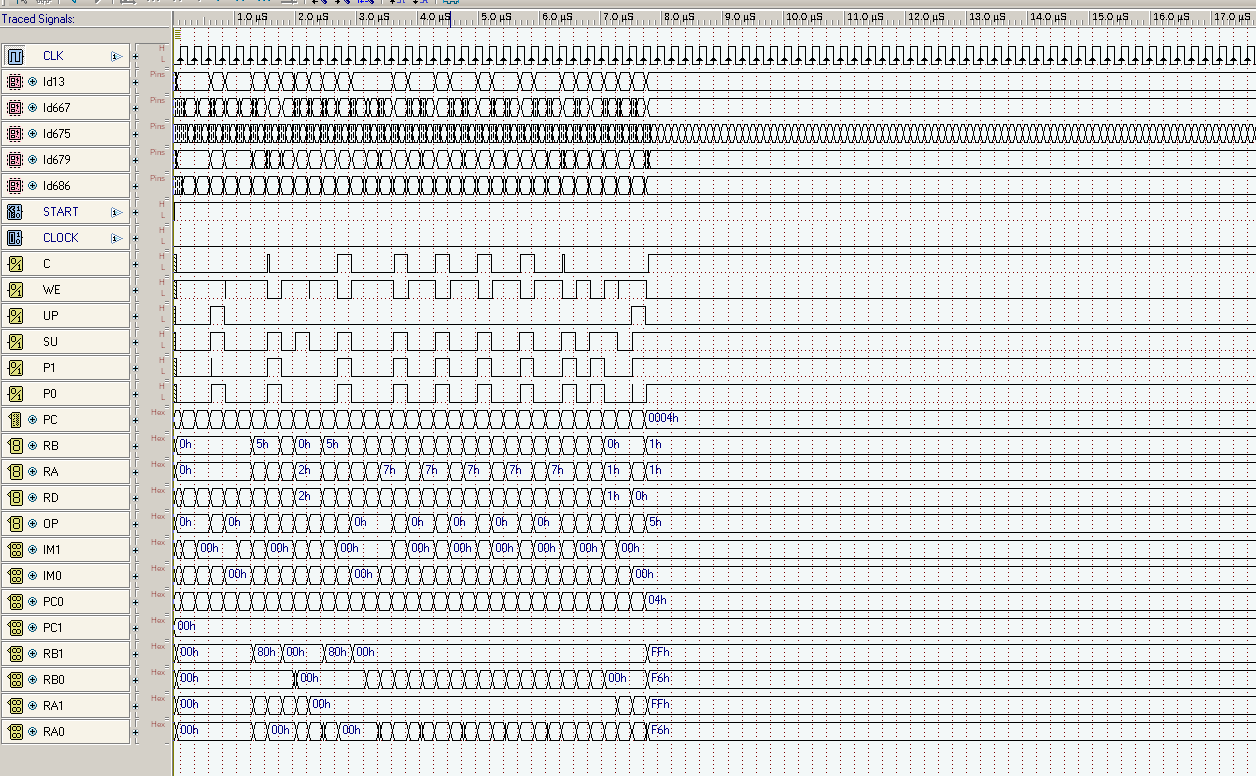
\includegraphics[width=.9\textwidth]{Projeto/images/program__mult_wave.png}
    \caption{Diagrama de onda para o programa Mult}\label{fig:program__mult_wave.png}
\end{figure}

\subsection{Divisão de Números sem Sinal}\label{sec:programs:divu}

Agora, para o programa de divisão de números sem sinal, o programa proposto
realiza a divisão de um número pelo outro, ambos representados sem sinal, e
retorna o valor da divisão no registrador \emph{R1}. Os valores de input para o
programa serão carregados nos registradores \emph{R2} e \emph{R3}, com valores
de $60$ e $12$, respectivamente. O resultado esperado da divisão será
$\frac{60}{12} = 5$, que, em hexadecimal, corresponde a $0x0005$.

O código do programa, e seus respectivos comentários, podem ser encontrados na
tabela~\ref{tab:programs:divu}.

\begin{table}[H]
    \centering
    \caption{Código para o programa \textbf{Divu}}
    \begin{tabular}{|l|l|l|l|}\hline
        \textbf{Endereço} & \textbf{Código Hexadecimal} & \textbf{Instrução} & \textbf{Comentário} \\\hline
        0x0000       & 0x0000 0010 & addi R1,R0,R0,0  & R1 = 0 ;; Resultado           \\\hline
        0x0001       & 0x003C 0020 & addi R2,R0,R0,60 & R2 = 60                       \\\hline
        0x0002       & 0x000C 0030 & addi R3,R0,R0,12 & R3 = 12                       \\\hline
        0x0003       & 0x0002 00FB & jal R15,Proc     & R15 = 0x0004; PC=Proc         \\\hline
        0x0004 Fim:  & 0x0000 1105 & beq R1,R1,0      & j Fim ;; mostra R1            \\\hline
        0x0005 Proc: & 0x0000 0040 & addi R4,R0,R0,0  & R4 = 0 ;; store the quotient  \\\hline
        0x0006       & 0x0007 230A & bgtu R3,R2,End   & Make sure R2 $>=$ R3          \\\hline
        0x0007 Loop: & 0x0000 3221 & subi R2,R2,R3,0  & R2 -= R3                      \\\hline
        0x0008       & 0x0001 0440 & addi R4,R4,R0,1  & R4 += 1                       \\\hline
        0x0009       & 0xFFFE 320A & bgtu R2,R3,Loop  & if (R2 $>$ R3) goto Loop      \\\hline
        0x000A       & 0x0003 3206 & bne  R2,R3,End   & if (R2 \!= R3) goto End       \\\hline
        0x000B       & 0x0001 0440 & addi R4,R4,R0,1  & R4 += 1                       \\\hline
        0x000C       & 0x0000 0020 & addi R2,R0,R0,0  & R2 = 0                        \\\hline
        0x000D End:  & 0x0000 0410 & addi R1,R4,R0,0  & R1 = R4 ;; get the quotient   \\\hline
        0x000E       & 0x0000 0F0C & jalr R0,R15,0    & Retorna resultado em R1       \\\hline
    \end{tabular}\label{tab:programs:divu}
\end{table}

Para a demonstração do programa funcionando, por favor conferir o vídeo no link:
\href{https://youtu.be/ZgymrJHToj8}{https://youtu.be/ZgymrJHToj8}

E, como requisitado, o diagrama de onda do programa pode ser visto na
figura~\ref{fig:program__divu_wave.png}. O processador conseguiu executar o
presente programa na máxima frequência de $4.35MHz$. Qualquer outra frequência
mais rápida que essa resulta em falha no funcionamento, e toda frequência menor
que essa resulta em um resultado sub-ótimo.

\begin{figure}[H]
    \centering
    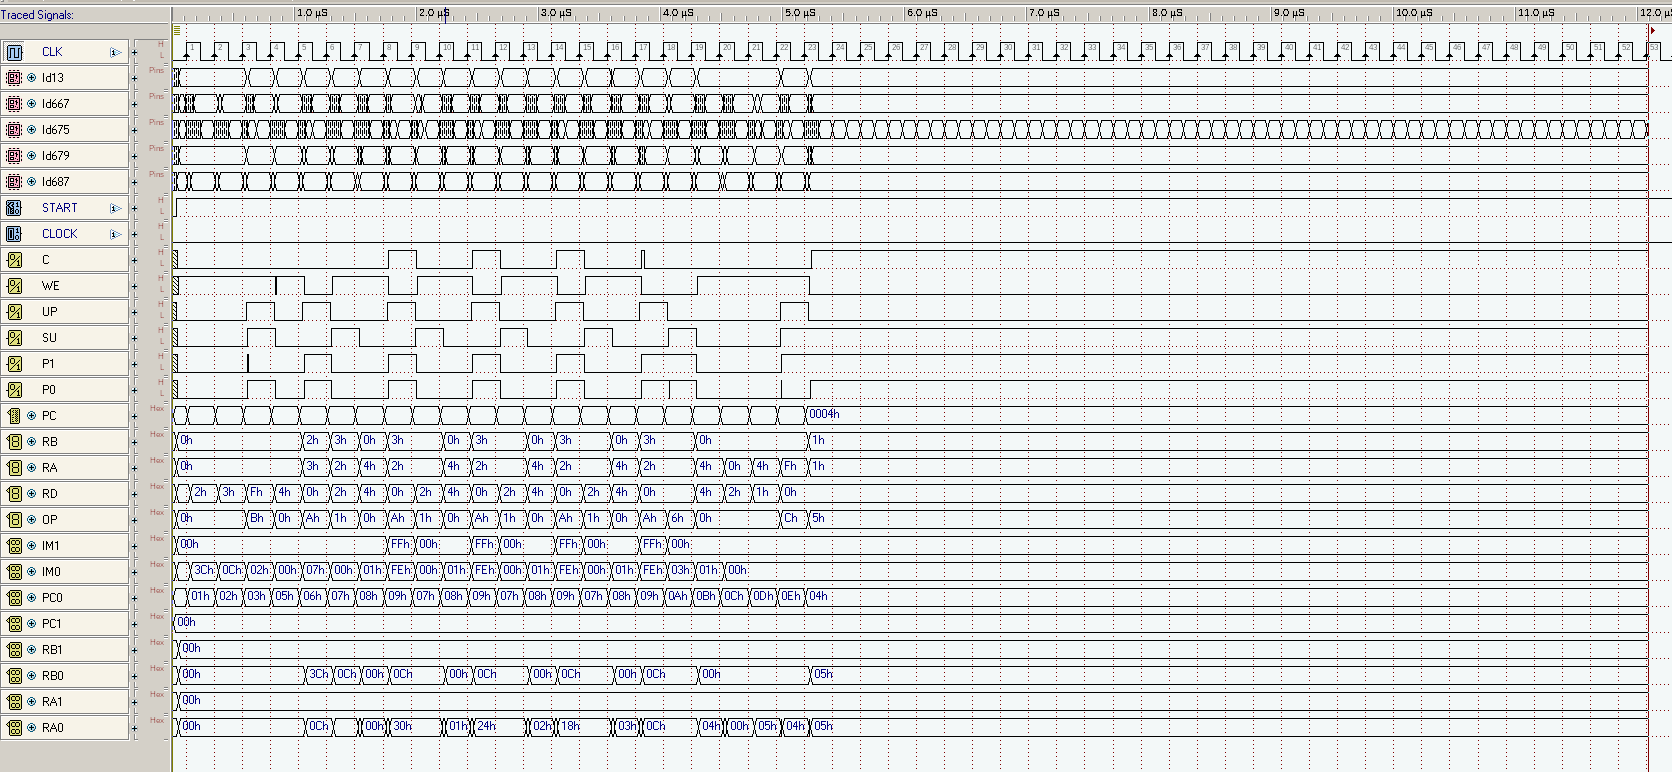
\includegraphics[width=.9\textwidth]{Projeto/images/program__divu_wave.png}
    \caption{Diagrama de onda para o programa Divu}\label{fig:program__divu_wave.png}
\end{figure}


\subsection{Divisão de Números com Sinal}\label{sec:programs:div}

Agora, para o programa de divisão de números com sinal, o programa proposto
realiza a divisão de um número pelo outro, ambos representados com sinal, e
retorna o valor da divisão no registrador \emph{R1}. Os valores de input para o
programa serão carregados nos registradores \emph{R2} e \emph{R3}, com valores
de $1337$ e $-42$, respectivamente. O resultado esperado da divisão será
$\frac{1337}{-42} = -31$, que, em hexadecimal, corresponde a $0xFFE1$. É
importante fazer a observação de que optamos por seguir o padão ANSI99 para a
divisão de números negativos. (A mesma divisão, utilizando o algotimo
implementado na linguagem \emph{Python}, por exemplo, retornaria $-32$).

O código do programa, e seus respectivos comentários, podem ser encontrados na
tabela~\ref{tab:programs:div}.

\begin{table}[H]
    \centering
    \caption{Código para o programa \textbf{Div}}
    \begin{tabular}{|l|l|l|l|}\hline
        % R4 = quociente
        % R2 = resto
        %  1337  42 = 001F
        % -1337  42 = FFE1
        %  1337 -42 = FFE1
        \textbf{Endereço} & \textbf{Código Hexadecimal} & \textbf{Instrução} & \textbf{Comentário} \\\hline
        0x0000         & 0x0000 0010 & addi R1,R0,R0,0      & R1 = 0 ;; Resultado          \\\hline
        0x0001         & 0x0539 0020 & addi R2,R0,R0,64     & R2 = 1337                    \\\hline
        0x0002         & 0xFFD6 0030 & addi R3,R0,R0,12     & R3 = -42                     \\\hline
        0x0003         & 0x0002 00FB & jal  R15,Proc        & R15 = 0x0004; PC=Proc        \\\hline
        0x0004 Fim:    & 0x0000 1105 & beq  R1,R1,0         & j Fim ;; mostra R1           \\\hline
        0x0005 Proc:   & 0x0000 0040 & addi R4,R0,R0,0      & R4 = 0 ;; store the quotient \\\hline
        0x0006         & 0x0000 0050 & addi R5,R0,R0,0      & R5 = 0 ;; division flag      \\\hline
        0x0007         & 0x0003 0209 & bgt  R2,R0,Apos      & if (R2 > R0) goto Apos       \\\hline
        0x0008         & 0x0000 2021 & subi R2,R0,R2,0      & R2 = -R2                     \\\hline
        0x0009         & 0x0001 0550 & addi R5,R5,R0,1      & R5 += 1                      \\\hline
        0x000A Apos:   & 0x0003 0309 & bgt  R3,R0,Div       & if (R3 > R0) goto Bpos       \\\hline
        0x000B         & 0x0000 3031 & subi R3,R0,R3,0      & R3 = -R3                     \\\hline
        0x000C         & 0x0001 0550 & addi R5,R5,R0,1      & R5 += 1                      \\\hline
        0x000D Div:    & 0x0000 3221 & subi R2,R2,R3,0      & R2 -= R3                     \\\hline
        0x000E         & 0x0003 2009 & bgt  R0,R2,Enddiv    & if (R2 > R0) goto Enddiv     \\\hline
        0x000F         & 0x0001 0440 & addi R4,R4,R0,1      & R4 += 1                      \\\hline
        0x0010         & 0xFFFD 000B & jal  R0,Div          & goto Div                     \\\hline
        0x0011 Enddiv: & 0x0000 3220 & addi R2,R2,R3,0      & R2 += R3                     \\\hline
        0x0012         & 0x0001 0660 & addi R6,R6,R0,1      & R6 = 1                       \\\hline
        0x0013         & 0x0002 6506 & bne  R5,R6,End       & if (R5 \!= R6) goto End      \\\hline
        0x0014         & 0x0000 4041 & subi R4,R0,R4,0      & R4 = -R4                     \\\hline
        0x0015 End:    & 0x0000 0410 & addi R1,R4,R0,0      & R1 = R4 ; save quotient      \\\hline
        0x0016         & 0x0000 0F0C & jalr R0,R15,0        & Retorna resultado em R1      \\\hline
    \end{tabular}\label{tab:programs:div}
\end{table}

Para a demonstração do programa funcionando, por favor conferir o vídeo no link:
\href{https://youtu.be/BimxtoXOGsk}{https://youtu.be/BimxtoXOGsk}

E, como requisitado, o diagrama de onda do programa pode ser visto na
figura~\ref{fig:program__div_wave.png}. O processador conseguiu executar o
presente programa na máxima frequência de $4.35MHz$. Qualquer outra frequência
mais rápida que essa resulta em falha no funcionamento, e toda frequência menor
que essa resulta em um resultado sub-ótimo.

\begin{figure}[H]
    \centering
    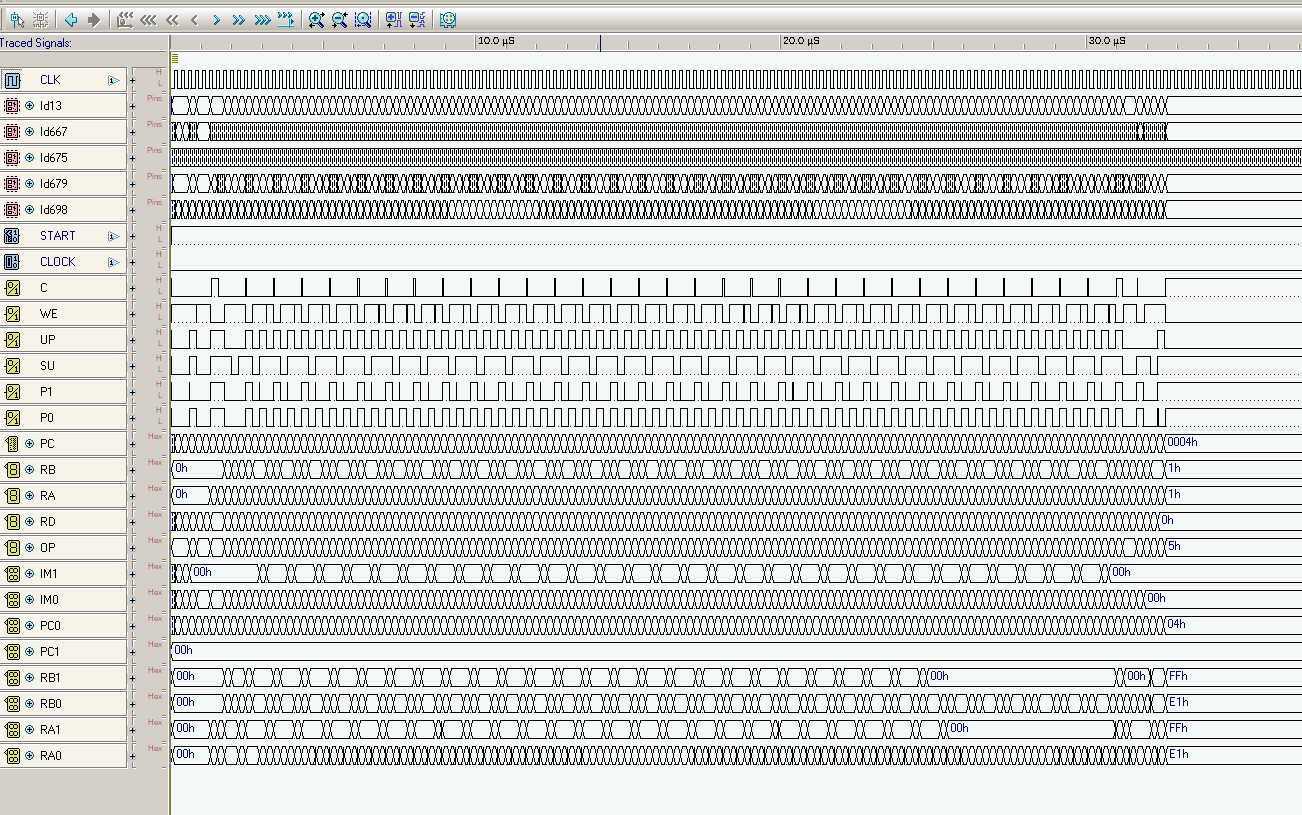
\includegraphics[width=.9\textwidth]{Projeto/images/program__div_wave.png}
    \caption{Diagrama de onda para o programa Div}\label{fig:program__div_wave.png}
\end{figure}

\subsection{Resto da Divisão de Números sem Sinal}\label{sec:programs:remu}

Agora, para o programa que computa do resto da divisão de números sem sinal, o
programa proposto realiza a divisão de um número pelo outro, ambos representados
sem sinal, e retorna o valor do resto da divisão no registrador \emph{R1}. Os
valores de input para o programa serão carregados nos registradores \emph{R2} e
\emph{R3}, com valores de $64$ e $12$, respectivamente. O resultado esperado do
resto da divisão será $4$, pois $64 = 12 * 5 + 4$. Como o resultado é dado em
hexadecimal, esse valor será de $0x0004$.

O código do programa, e seus respectivos comentários, podem ser encontrados na
tabela~\ref{tab:programs:remu}.

\begin{table}[H]
    \centering
    \caption{Código para o programa \textbf{Remu}}
    \begin{tabular}{|l|l|l|l|}\hline
        \textbf{Endereço} & \textbf{Código Hexadecimal} & \textbf{Instrução} & \textbf{Comentário} \\\hline
        0x0000       & 0x0000 0010 & addi R1,R0,R0,0  & R1 = 0 ;; Resultado           \\\hline
        0x0001       & 0x0040 0020 & addi R2,R0,R0,64 & R2 = 64                       \\\hline
        0x0002       & 0x000C 0030 & addi R3,R0,R0,12 & R3 = 12                       \\\hline
        0x0003       & 0x0002 00FB & jal R15,Proc     & R15 = 0x0004; PC=Proc         \\\hline
        0x0004 Fim:  & 0x0000 1105 & beq R1,R1,0      & j Fim ;; mostra R1            \\\hline
        0x0005 Proc: & 0x0000 0040 & addi R4,R0,R0,0  & R4 = 0 ;; store the quotient  \\\hline
        0x0006       & 0x0007 230A & bgtu R3,R2,End   & Make sure R2 $>=$ R3          \\\hline
        0x0007 Loop: & 0x0000 3221 & subi R2,R2,R3,0  & R2 -= R3                      \\\hline
        0x0008       & 0x0001 0440 & addi R4,R4,R0,1  & R4 += 1                       \\\hline
        0x0009       & 0xFFFE 320A & bgtu R2,R3,Loop  & if (R2 > R3) goto Loop        \\\hline
        0x000A       & 0x0003 3206 & bne  R2,R3,End   & if (R2 \!= R3) goto End       \\\hline
        0x000B       & 0x0001 0440 & addi R4,R4,R0,1  & R4 += 1                       \\\hline
        0x000C       & 0x0000 0020 & addi R2,R0,R0,0  & R2 = 0                        \\\hline
        0x000D End:  & 0x0000 0210 & addi R1,R2,R0,0  & R1 = R2 ;; get the remainder  \\\hline
        0x000E       & 0x0000 0F0C & jalr R0,R15,0    & Retorna resultado em R1       \\\hline
    \end{tabular}\label{tab:programs:remu}
\end{table}

Para a demonstração do programa funcionando, por favor conferir o vídeo no link:
\href{https://youtu.be/OMpzPPJSW2Q}{https://youtu.be/OMpzPPJSW2Q}

E, como requisitado, o diagrama de onda do programa pode ser visto na
figura~\ref{fig:program__remu_wave.png}. O processador conseguiu executar o
presente programa na máxima frequência de $4.35MHz$. Qualquer outra frequência
mais rápida que essa resulta em falha no funcionamento, e toda frequência menor
que essa resulta em um resultado sub-ótimo.

\begin{figure}[H]
    \centering
    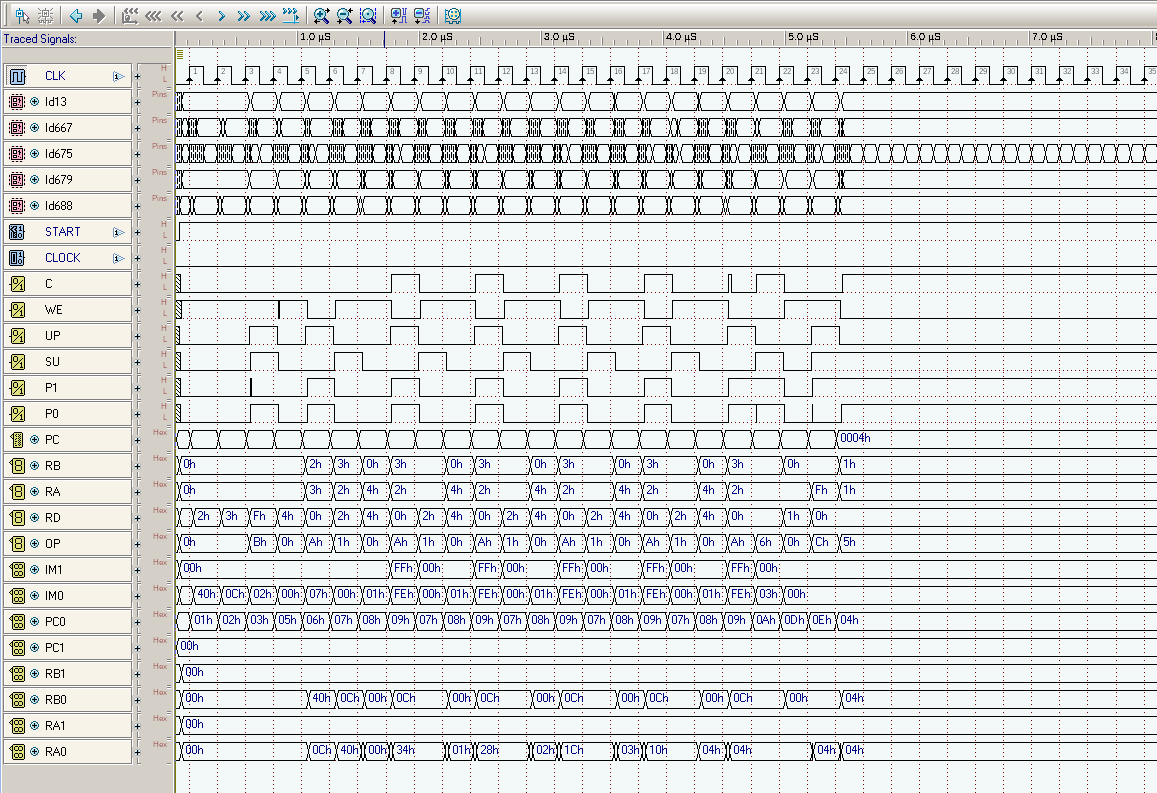
\includegraphics[width=.9\textwidth]{Projeto/images/program__remu_wave.png}
    \caption{Diagrama de onda para o programa Remu}\label{fig:program__remu_wave.png}
\end{figure}


\subsection{Resto da Divisão de Números com Sinal}\label{sec:programs:rem}

Agora, para o programa que computa do resto da divisão de números com sinal, o
programa proposto realiza a divisão de um número pelo outro, ambos representados
com sinal, e retorna o valor do resto da divisão no registrador \emph{R1}. Os
valores de input para o programa serão carregados nos registradores \emph{R2} e
\emph{R3}, com valores de $1337$ e $-42$, respectivamente. O resultado esperado
do resto da divisão será $35$, pois estamos usando o padrão ANSI99 para
realizarmos as divisões. Como o resultado é dado em hexadecimal, esse valor será
de $0x0023$.

O código do programa, e seus respectivos comentários, podem ser encontrados na
tabela~\ref{tab:programs:rem}.

\begin{table}[H]
    \centering
    \caption{Código para o programa \textbf{Rem}}
    \begin{tabular}{|l|l|l|l|}\hline
        % R4 = quociente
        % R2 = resto
        %  1337  42 = 001F
        % -1337  42 = FFE1
        %  1337 -42 = FFE1
        \textbf{Endereço} & \textbf{Código Hexadecimal} & \textbf{Instrução} & \textbf{Comentário} \\\hline
        0x0000         & 0x0000 0010 & addi R1,R0,R0,0      & R1 = 0 ;; Resultado          \\\hline
        0x0001         & 0x0539 0020 & addi R2,R0,R0,64     & R2 = 1337                    \\\hline
        0x0002         & 0xFFD6 0030 & addi R3,R0,R0,12     & R3 = -42                     \\\hline
        0x0003         & 0x0002 00FB & jal  R15,Proc        & R15 = 0x0004; PC=Proc        \\\hline
        0x0004 Fim:    & 0x0000 1105 & beq  R1,R1,0         & j Fim ;; mostra R1           \\\hline
        0x0005 Proc:   & 0x0000 0040 & addi R4,R0,R0,0      & R4 = 0 ;; store the quotient \\\hline
        0x0006         & 0x0000 0050 & addi R5,R0,R0,0      & R5 = 0 ;; division flag      \\\hline
        0x0007         & 0x0003 0209 & bgt  R2,R0,Apos      & if (R2 > R0) goto Apos       \\\hline
        0x0008         & 0x0000 2021 & subi R2,R0,R2,0      & R2 = -R2                     \\\hline
        0x0009         & 0x0001 0550 & addi R5,R5,R0,1      & R5 += 1                      \\\hline
        0x000A Apos:   & 0x0003 0309 & bgt  R3,R0,Div       & if (R3 > R0) goto Bpos       \\\hline
        0x000B         & 0x0000 3031 & subi R3,R0,R3,0      & R3 = -R3                     \\\hline
        0x000C         & 0x0001 0550 & addi R5,R5,R0,1      & R5 += 1                      \\\hline
        0x000D Div:    & 0x0000 3221 & subi R2,R2,R3,0      & R2 -= R3                     \\\hline
        0x000E         & 0x0003 2009 & bgt  R0,R2,Enddiv    & if (R2 > R0) goto Enddiv     \\\hline
        0x000F         & 0x0001 0440 & addi R4,R4,R0,1      & R4 += 1                      \\\hline
        0x0010         & 0xFFFD 000B & jal  R0,Div          & goto Div                     \\\hline
        0x0011 Enddiv: & 0x0000 3220 & addi R2,R2,R3,0      & R2 += R3                     \\\hline
        0x0012         & 0x0001 0660 & addi R6,R6,R0,1      & R6 = 1                       \\\hline
        0x0013         & 0x0002 6506 & bne  R5,R6,End       & if (R5 \!= R6) goto End      \\\hline
        0x0014         & 0x0000 4041 & subi R4,R0,R4,0      & R4 = -R4                     \\\hline
        0x0015 End:    & 0x0000 0210 & addi R1,R2,R0,0      & R1 = R2 ; save remainder     \\\hline
        0x0016         & 0x0000 0F0C & jalr R0,R15,0        & Retorna resultado em R1      \\\hline
    \end{tabular}\label{tab:programs:rem}
\end{table}

Para a demonstração do programa funcionando, por favor conferir o vídeo no link:
\href{https://youtu.be/-2xW0z4dV00}{https://youtu.be/-2xW0z4dV00}

E, como requisitado, o diagrama de onda do programa pode ser visto na
figura~\ref{fig:program__rem_wave.png}. O processador conseguiu executar o
presente programa na máxima frequência de $4.35MHz$. Qualquer outra frequência
mais rápida que essa resulta em falha no funcionamento, e toda frequência menor
que essa resulta em um resultado sub-ótimo.

\begin{figure}[H]
    \centering
    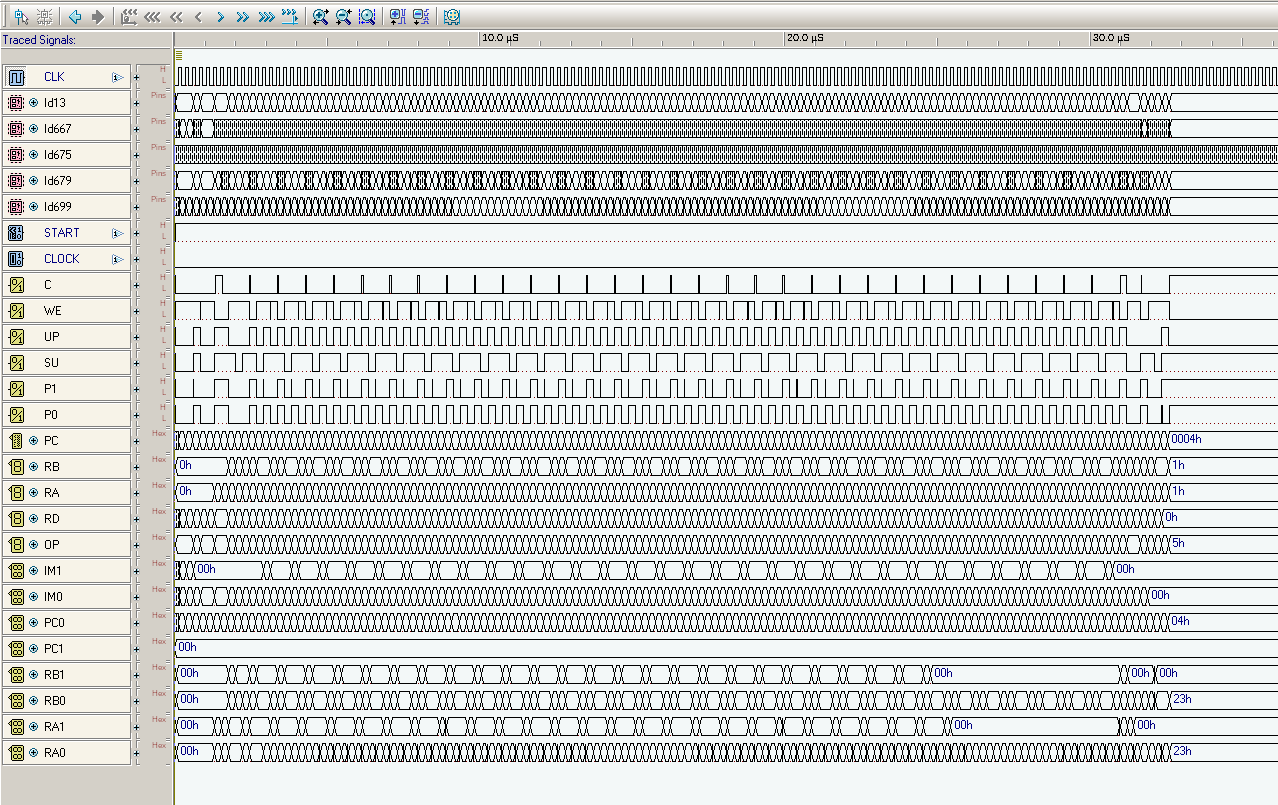
\includegraphics[width=.9\textwidth]{Projeto/images/program__rem_wave.png}
    \caption{Diagrama de onda para o programa Rem}\label{fig:program__rem_wave.png}
\end{figure}

\subsection{Encontrando o primeiro primo em um intervalo}\label{sec:programs:prime}

Para essa questão, desejamos encontar o primeiro número primo existente em um
intervalo. E, caso não haja nenum número primo, retornar zero como resultado.
Usaremos o código apresentado na seção~\ref{sec:programs:remu} como base para
encontrarmos se um número é divisor de outro ou não. O código em Assembly
seguirá o seguinte algoritmo demonstrado em \emph{Python}.

\begin{python}
def is_prime(n: int) -> bool:
    for j in range(2, n):
        if n%j == 0:
            return False
    return True

def find_first_prime(x: int, y: int) -> int:
    for i in range(x, y+1):
        if is_prime(i):
            return i
    return 0
\end{python}


\begin{table}[H]
    \centering
    \caption{Código para o programa \textbf{Primo}}
    \begin{tabular}{|l|l|l|l|}\hline
        \textbf{Endereço} & \textbf{Código Hexadecimal} & \textbf{Instrução} & \textbf{Comentário} \\\hline
        0x0000 & 0x0000 0010 & addi r1 r0 r0 0   & ----------------------------\\\hline
        0x0001 & 0x0036 0020 & addi r2 r0 r0 54  & ----------------------------\\\hline
        0x0002 & 0x0064 0030 & addi r3 r0 r0 100 & ----------------------------\\\hline
        0x0003 & 0x0005 00FB & jal r15 5         & ----------------------------\\\hline
        0x0004 & 0x0000 2010 & addi r1 r0 r2 0   & ----------------------------\\\hline
        0x0005 & 0x0000 1105 & beq r1 r1 0       & ----------------------------\\\hline
        0x0006 & 0x0001 0220 & addi r2 r2 r0 1   & ----------------------------\\\hline
        0x0007 & 0xfffe 3209 & bgt r2 r3 -2      & ----------------------------\\\hline
        0x0008 & 0x0000 2040 & addi r4 r0 r2 0   & ----------------------------\\\hline
        0x0009 & 0x0002 0050 & addi r5 r0 r0 2   & ----------------------------\\\hline
        0x000A & 0x0005 000B & jal r0 5          & ----------------------------\\\hline
        0x000b & 0xfffb 0405 & beq r4 r0 -5      & ----------------------------\\\hline % register R8 is 'n' the number to find if is prime or not
        0x000c & 0x0001 0550 & addi r5 r5 r0 1   & ----------------------------\\\hline
        0x000d & 0x0000 2040 & addi r4 r0 r2 0   & ----------------------------\\\hline
        0x000e & 0xfff6 4505 & beq r5 r4 -10     & ----------------------------\\\hline
        0x000f & 0x0000 5441 & subi r4 r4 r5 0   & ----------------------------\\\hline
        0x0010 & 0xfffb 4009 & bgt r0 r4 -5      & ----------------------------\\\hline
        0x0011 & 0xfffa 0405 & beq r4 r0 -6      & ----------------------------\\\hline
        0x0012 & 0xfffd 000B & jal r0 -3         & ----------------------------\\\hline
        0x0013 & 0x0000 0F0C & jalr r0 r15 0     & ----------------------------\\\hline
    \end{tabular}\label{tab:programs:primo}
\end{table}



Para a demonstração do programa funcionando, por favor conferir o vídeo no link:
\href{https://youtu.be/nBpRLZitRZc}{https://youtu.be/nBpRLZitRZc}

E, como requisitado, o diagrama de onda do programa pode ser visto na
figura~\ref{fig:program__primo_wave.png}. O processador conseguiu executar o
presente programa na máxima frequência de $4.35MHz$. Qualquer outra frequência
mais rápida que essa resulta em falha no funcionamento, e toda frequência menor
que essa resulta em um resultado sub-ótimo.

\begin{figure}[H]
    \centering
    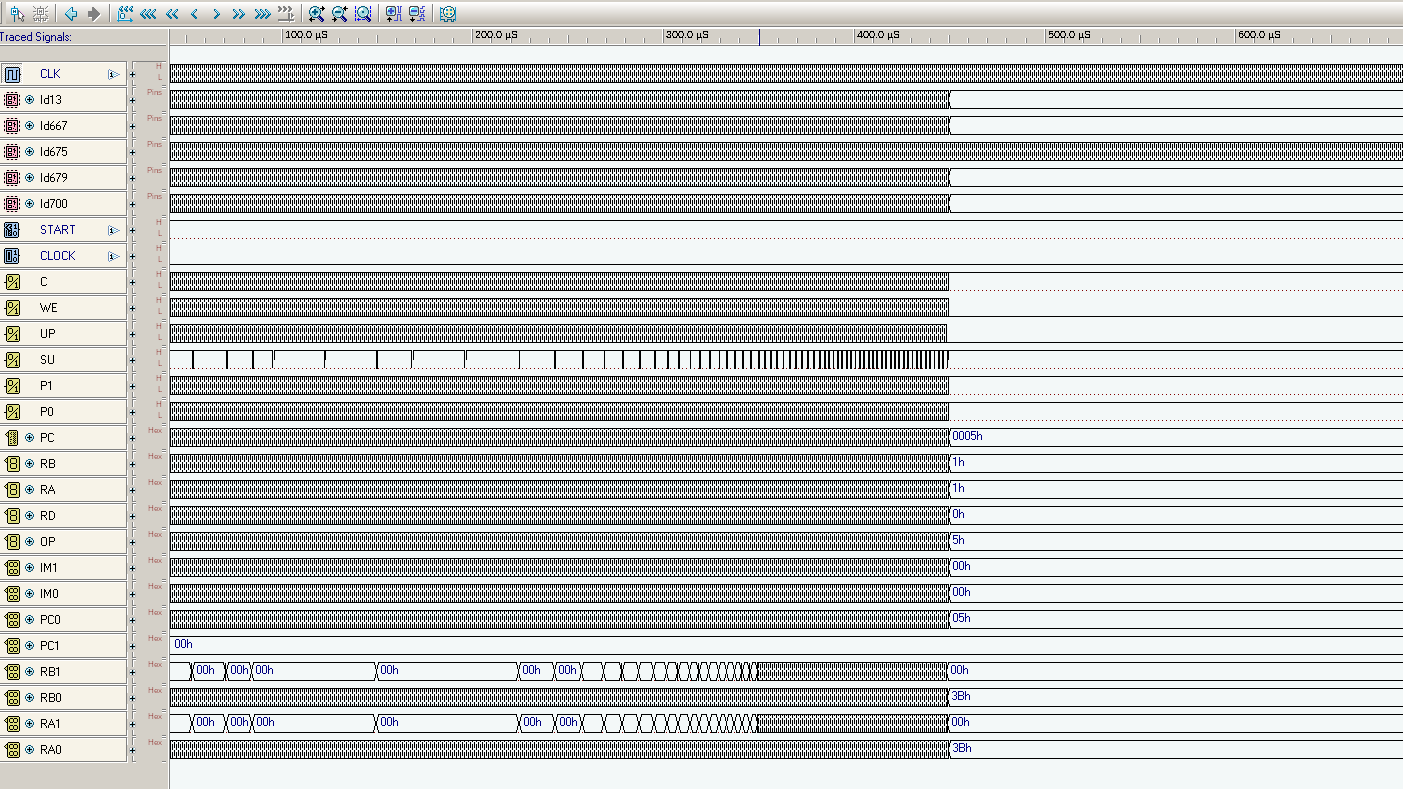
\includegraphics[width=.9\textwidth]{Projeto/images/program__primo_wave.png}
    \caption{Diagrama de onda para o programa Primo}\label{fig:program__primo_wave.png}
\end{figure}


\subsection{Maior frequência do ZeptoProcessador-III}\label{sec:programs:frequency}

Como requisitado no enunciado do projeto, abordaremos agora a questão da
frequência máxima de operação do ZeptoProcessador-III. O resultado encontrado
para a maior frequência operação correra do ZeptoProcessador-III foi de
$4.35MHz$ (um comprimento de onda de $230nS$).

O limitante para uma maior frequência de operação é o tempo para a obtenção dos
resultados da operação atual sendo processada, pois, para completar um ciclo de
instrução, pode ser levado um tempo ``X''. Entretanto, caso a frequência
ultrapasse as limitações do processador teremos que antes mesmo da finalização
de uma instrução outra já estará sendo executada. Isso acarretará em um estado
inconsistente do circuito lógico do processador e, por consequência, em um
funcionamento incorreto do mesmo.

% \section{Análise dos Resultados}\label{sec:resultados}

% Passaremos a analisar individualmente cada um dos tópicos anteriores, levantando
% observações pertinentes para cada um deles.

% \subsection{Análise do tópico~\ref{sec:2.1}}\label{sec:analise2.1}

% \textbf{TODO}

% \subsection{Análise do tópico~\ref{sec:2.2}}\label{sec:analise2.2}

% \textbf{TODO}

% \subsection{Análise do tópico~\ref{sec:2.3}}\label{sec:analise2.3}

% \textbf{TODO}

% \subsection{Análise do tópico~\ref{sec:2.4}}\label{sec:analise2.4}

% \textbf{TODO}

\section{Conclusão}\label{sec:Conclusao}

Com esse projeto pudemos ver todo o processo para desenvolvimento de um
processador, mesmo que um simples. O circuito lógico necessário para tal
construção provou-se complexo, como mencionado no início desse relatório. Por
meio da utilização de portas lógicas pudtemos desenvolver abstrações mais
complexas, como multiplexadores, somadores, \emph{Flip-flops}, e, subindo no
nível de abstrações, finalmente pudemos implementar registradores de instrução,
uma memória de instrução suficientemente grande para comportar $32$ \emph{bits}
de instrução, um banco de registradores de $16$ \emph{bits}, e toda uma lógica
para interpretação de códigos de operação para funcionamento do processador
condicionado ao código inserido pelo usuário.

Como pudemos constatar na seção~\ref{sec:programs:frequency}, o
ZeptoProcessador-III é limitado a uma frequência máxima de operação de
$4.35MHz$, demonstrando com o atraso de portas lógicas acabam se somando e
impactando na velocidade do circuito final.

\bibliographystyle{sbc}
\bibliography{relatorio}  %Aqui é a definição do arquivo .bib a ser usado pelas referências

\end{document}
